\documentclass[11pt, a4paper]{article}
\usepackage[a4paper, margin = 0.7in]{geometry}
\usepackage{graphicx}
\usepackage{amsmath}
\usepackage{listings}
\usepackage{url}

\title{EE2703 Assignment 6 : Tubelight Simulation}
\author{Aman Kumar EE19B066}
\date{April 17, 2021}

\begin{document}

\maketitle

\section{The Assignment}
\subsection{Introduction}
    In this assignment we have to simulate a tubelight. We use a 1-Dimensional model of the tubelight. A uniform electric field is present, that accelerates electrons. Electrons are emitted by the cathode with \textbf{zero energy}(i.e. zero velocity), and accelerated in this field. When they get beyond a \textbf{threshold energy E0}(i.e. threshold velocity \textit{u0}), they can drive atoms to excited states. The relaxation of these atoms results in light emission. In our model, we have to assume that the relaxation is immediate. The collision is inelastic, and thus the electron loses all its energy after the collision and the process starts again. The electrons reaching the anode are lost.
    
    One of the important things that we learn in this assignment is learning to work with index vectors. We also learn how to run simulations in time.
\subsection{Things to do}
    Mainly the following things are asked in this assignment:
    \begin{itemize}
        \item Electron density plot
        \item Population plot of light intensity. i.e. Light intensity as a function of space after the process reaches steady state.
        \item Electron phase plot.
        \item Intensity data table.
    \end{itemize}
\section{Assignment questions}
\subsection{The simulation universe}
    \begin{itemize}
        \item The tube is divided into \textbf{n} sections.
        \item In each time instant, on average \textbf{M} electrons are injected with a standard deviation of \textbf{Msig}.
        \item We run the simulation for \textbf{nk} turns. 
        \item The electrons are unable to excite the atoms till they have a threshold velocity of \textbf{u0}.
        \item  Beyond this velocity, there is a probability \textbf{p} in each turn that a collision will occur and an atom excited.
    \end{itemize}
    The electron’s velocity reduces to zero if it collides.
    
    Each of six parameters have default values, and if the user wants to update some parameter(s) then all 6 parameters have to passed with updated values. They should be passed in this order-
    \begin{verbatim}
                                    n M Msig nk u0 p
    \end{verbatim}
     If the arguments are not passed correctly, then the default values are taken for \textbf{all} of them. The python code snippet for doing this:
    \begin{verbatim}
if len(argv) != 7:                      #Checking if all 6 parameters have been passed
    n,M,Msig,nk,u0,p = 100,5,2,500,5,0.25    #Default values
    print("Usage: python",argv[0],"n M Msig nk u0 p")
    print("The program will run using default parameter values.")
else:
    #Updating the values user has passed
    n = int(argv[1])        #spatial frid size             
    M = int(argv[2])        #avg number of electrons injected per turn
    Msig = float(argv[3])   #stddev of number of electrons injected each turn
    nk = int(argv[4])       #number of turns
    u0 = float(argv[5])     #threshold velocity
    p = float(argv[6])      #probability of ionization
    \end{verbatim}
\subsection{Vectors to store information}
    We need vectors to hold the electron information. We need vectors for:
    \begin{itemize}
        \item Electron position xx
        \item Electron velocity u
        \item Displacement in current turn dx
    \end{itemize}
    We also need vectors to accumulate information as part of simulation. Three vectors are needed for storing:
    \begin{itemize}
        \item Intensity of emitted light, I
        \item Electron position, X
        \item Electron velocity, V
    \end{itemize}
    \begin{verbatim}
#Creating vectors to hold the electron information
xx = np.zeros(n*M)                  #Electron position
u = np.zeros(n*M)                   #Electron velocity
dx = np.zeros(n*M)                  #Displacement in current turn
#Lists to accumulate information as part of the simulation
I = []                              #Intensity of emitted light
X = []                              #Electron position
V = []                              #Electron velocity        
    \end{verbatim}
\subsection{The Loop}
    This is the main loop of the program. It performs the simulation and Saves the Intensity, Position and Velocity data in I, X, V respectively. We are assuming that the Electric field creates an acceleration of 1. Hence, the displacement of the $i^{th}$ electron is given by
    \begin{equation*}
        dx_i = u_i\Delta t + \frac{1}{2}a(\Delta t)^2 = u_i + 0.5
    \end{equation*}
    \begin{verbatim}
ii = np.where(xx > 0)              #Finding indices of existing electrons
for k in range(nk):
    #ii = np.where(xx > 0)
    dx[ii] = u[ii] + 0.5           #Finding displacement for the electrons in this turn
    xx[ii] = xx[ii] + dx[ii]       #Updating the electron position
    u[ii] = u[ii] + 1              #Updating velocity.(acceleration = 1 unit) 
    
    jj = np.where(xx >= n)         #Electrons that have reached Anode are lost.
    xx[jj], dx[jj], u[jj] = 0,0,0  #Resetting there position, velocity and displacement
    
    kk = np.where(u >= u0)         #Finding electrons having atleast threshold energy
    ll = np.where(np.random.rand(len(kk[0]))<=p)
    kl = kk[0][ll]                 #Electrons at these indices will suffer collision
    
    u[kl] = 0                      #After inelastic collision they lose all energy
    xx[kl] = xx[kl] - dx[kl]*rd.random()
    I.extend(xx[kl].tolist())      #Light is emitted where collision happens.
    
    m = round(pl.randn()*Msig + M)    #Numner of electrons to be injected
    zz = np.where(xx == 0)         #Finding available space in the array.
    xx[zz[0][:m]] = 1              #Newly injected electrons are at position 1
    dx[zz[0][:m]] = 0              #Newly injected electrons have displacement = 0          
    u[zz[0][:m]] = 0               #Newly injected electrons have velocity = 0
    
    ii = np.where(xx > 0)          #Existing elecrons
    X.extend(xx[ii].tolist())      #Adding there position to X
    V.extend(u[ii].tolist())       #Adding there velocity to V
    \end{verbatim}
\section{Plots and Results(\textit{Parameters} : 100 5 2 500 5 0.25)}
\subsection{Electron density}
    The number of electrons between i and i+1. We do this using the \texttt{hist} function. The position data is accumulated in the vector \texttt{X}.
    \begin{verbatim}
pl.hist(X,n)
pl.title("Population plot for Electron Density")
    \end{verbatim}
    \begin{figure}[!h]
        \centering
        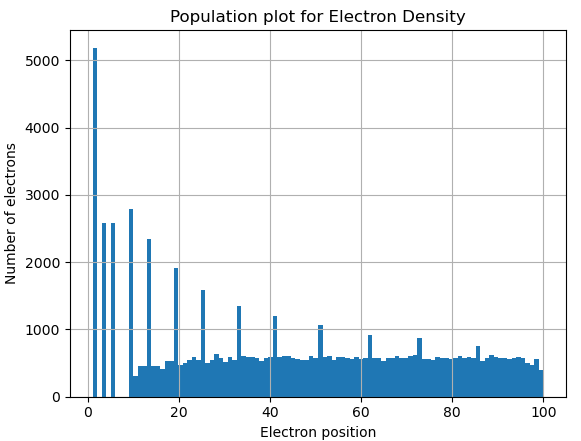
\includegraphics[scale = 0.69]{Figure 1.png}
        \caption{Electron Density}
        \label{fig:my_label}
    \end{figure}
\subsection{Light Intensity}
    The intensity data is accumulated in the vector \texttt{I}. That is it stores the positions where excitation happened after collision. These positions are stored the number of times a collision happens there.
    \begin{verbatim}
count,bins,rec=pl.hist(I,n)
pl.title("Population plot for Light Intensity")
    \end{verbatim}
    \begin{figure}[!h]
        \centering
        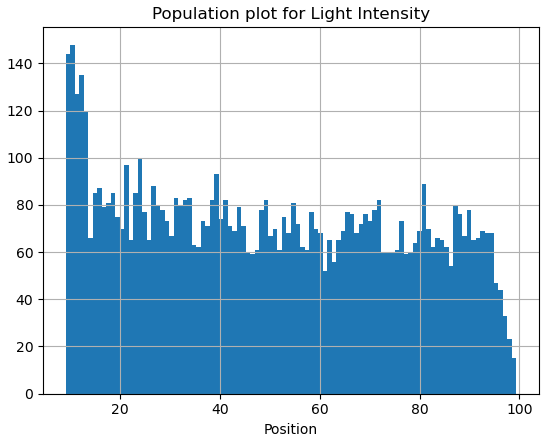
\includegraphics[scale = 0.67]{Figure 2.png}
        \caption{Light Intensity}
        \label{fig:my_label}
    \end{figure}
\subsection{Electron phase space}
    For each electron we plot a “X” corresponding to $x = x_i$, $y = v_i$.
    \begin{verbatim}
pl.scatter(X,V,marker="x")
pl.title("Electron Phase space")
    \end{verbatim}
    \begin{figure}[!h]
        \centering
        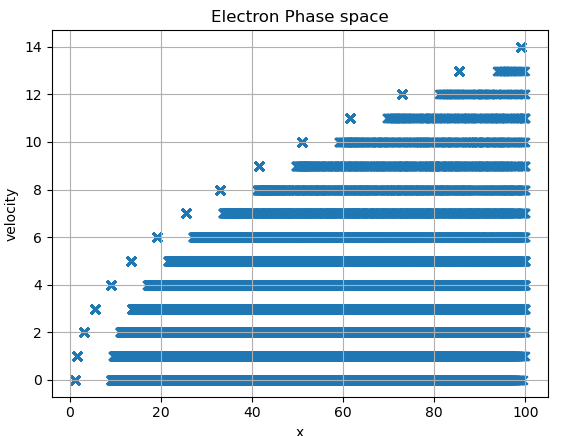
\includegraphics[scale = 0.67]{Figure 3.png}
        \caption{Electron phase space}
        \label{fig:my_label}
    \end{figure}
\subsection{Intensity Table}
    We need to print the population count against average bin positions.Python code snippet for printing the intensity table.
    \begin{verbatim}
xpos = 0.5*(bins[0:-1]+bins[1:])    #Converting bin positions to mid point values
print("\nIntensity data:\n")
print("\txpos\tcount")
ogm=np.c_[xpos, count]              #Concatenating the xpos and count vectors column-wise
s1 = str(ogm)
s2 = s1.replace('], [','\n')
s3 = s2.replace('[', '')
s4 = s3.replace(']','')
s5 = s4.replace(', ','\t')
print(s5)
    \end{verbatim}
    An example run of the program with intensity table:
    \begin{figure}[!h]
        \centering
        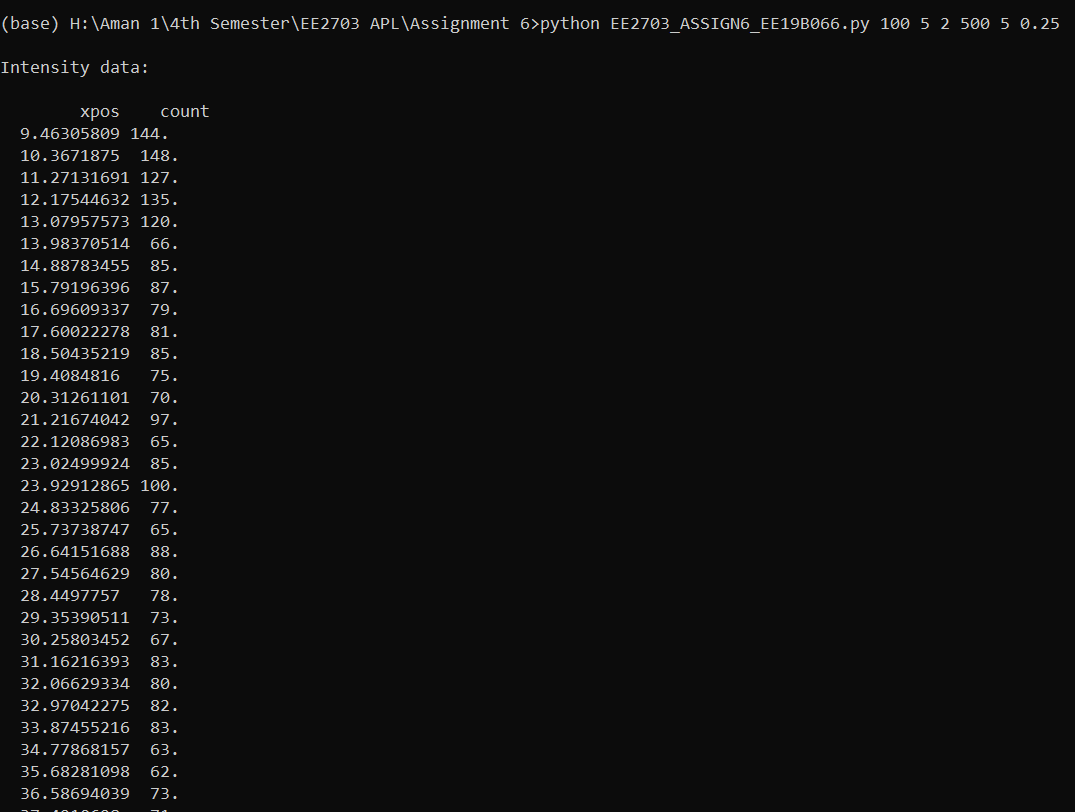
\includegraphics[scale = 0.6]{Figure 4.png}
        \caption{Example Run}
        \label{fig:my_label}
    \end{figure}
\subsection{Some more plots}
    I am plotting the above three plots again, this time with-
    \begin{verbatim}
        u0 = 7
        p = 0.75
        All other parameters are kept as it is
    \end{verbatim}
    \begin{figure}[!h]
        \centering
        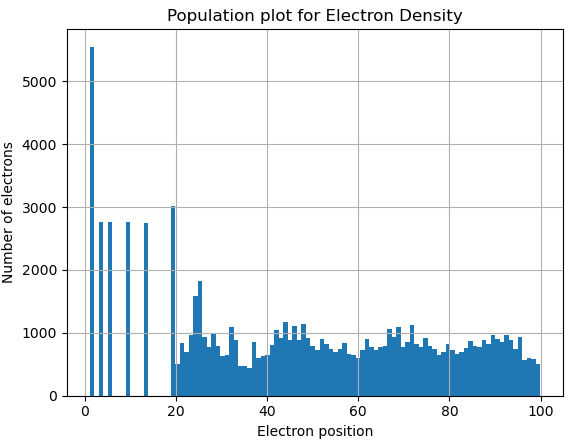
\includegraphics[scale = 0.6]{Figure 5.png}
        \caption{Electron density}
        \label{fig:Figure 5}
    \end{figure}
    \begin{figure}[!h]
        \centering
        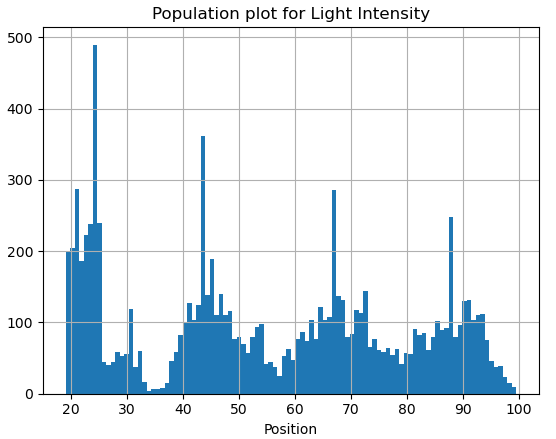
\includegraphics[scale = 0.65]{Figure 6.png}
        \caption{Light Intensity}
        \label{fig:Figure 6}
    \end{figure}
    \begin{figure}[!h]
        \centering
        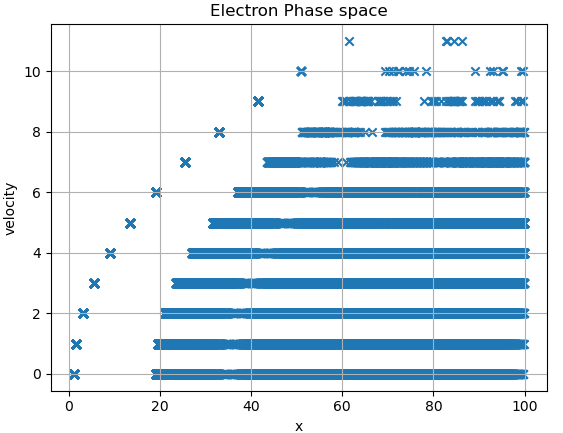
\includegraphics[scale = 0.6]{Figure 7.png}
        \caption{Electron phase space}
        \label{fig:Figure 7}
    \end{figure}
    This time in the Light Intensity plot, we can observe some \textit{dark spaces} in between $x = 30$ and $x = 40$, between $x = 50$ and $x = 60$.
\section{Conclusion}
    In this week we used for python for simulations in time. We learnt to work with index vectors. We simulated the motion of electrons in a tubelight( 1 D), and also the illumination. We tried to find the \textit{dark places}. With the parameter values $u0 = 7$ and $p = 0.75$, we got some dark places. In this the tubelight is dark in more of the initial region i.e. till around $x = 20$ there is no illumination.
\end{document}
